\section{System Analysis}\label{sec:system}
\vspace{-0.2cm} Sensors and actuators are hardware elements that govern the execution of cyber-physical systems in terms of how well it performs and what it is capable of. Understanding the limitations in hardware is a key step to designing systems that efficiently meet specifications. In addition, to enable smarter controller design, whilst analysing the physical Kobuki, comparisons were also drawn with the simulation environment, which is based on a physical model that simulates rigid body dynamics and render them in 3D \cite[p.~30]{labguide}.

\subsection{Kobuki Sensors and Actuators}
%A basic description of the sensor data available to myRIO and how it was used in your algorithm
\vspace{-0.2cm} With a variety of sensors available on the Kobuki as shown in Figure \ref{fig:kobuki_sensors}, we chose to use applicable sensors for our obstacle navigation. Table \ref{table:kobuki_sensors} shows the sensors we used in our design and the obstacle course specifications that the sensors will help achieve. The wheel drop sensors and bumpers are both triggered as boolean outputs when the requirement of the wheel touching the ground or bumper uncollided is no longer true. The cliff sensor will avoid cliffs deeper than 5cm \cite{kobuki_datasheet}, the sensor range is 2 - 15cm \cite{kobukisensors}.
\begin{figure}[H]
    \centering
    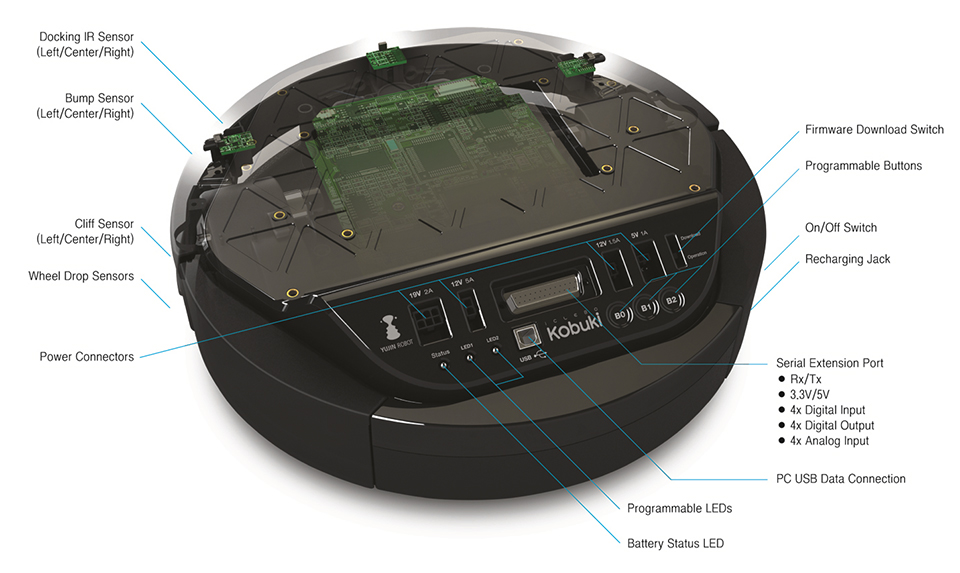
\includegraphics[width=12cm]{Images/kobuki_spec.jpg}
    \caption{Angle view of Kobuki with sensors labelled \cite{kobuki_spec_pic}}
    \label{fig:kobuki_sensors}
\end{figure}
\begin{table}[H]
\begin{center}
\begin{tabular}{ |l|c|c|c| } 
    \hline
    \textbf{Sensor} & \textbf{Number} & \textbf{Target Specification} & \textbf{Output} \\ 
    \hline
    Wheel Drop Sensor & 2 (left, right) & Maintain ground contact & Boolean\\
    \hline
    Cliff Sensor & 3 (left, center, right) & Hill climb edge avoidance & Boolean and Raw\\
    \hline
    Bumper & 3 (left, center, right) & Object avoidance & Boolean\\
    \hline
\end{tabular}
\caption{Kobuki Sensors} \label{table:kobuki_sensors}
\end{center}
\end{table}
\vspace{-0.5cm}
The Kobuki polls the sensors at 50Hz and returns the above sensor data as default ``Basic Sensor Data" in the form of a hexadecimal bytestream \cite{kobukisensors}. These sensors were also available on the simulation robot model. In addition to direct sensor data, the Kobuki also receives information on distance travelled (in mm) and angle rotated (in degrees) since origin. Compared to the simulation output, the real distance is signed and has angles unwrapped within $(-180^\circ, 180^\circ)$. The distance travelled is derived from the wheel movement so if the wheels were slipping, the reported distance travelled will still increase. The simulation only records the actual distance moved by the robot \cite[p.~37]{labguide}. The maximum rotational velocity is $180^\circ$/s (anything above $110^\circ$ will see degraded gyro performance) and the maximum translational velocity is 70cm/s \cite{kobuki_datasheet}. 

\subsection{Accelerometer ADXL330} \label{sec:acc}
\vspace{-0.2cm} In order to detect inclination and reorient the Kobuki on an incline, we used the accelerometer on the myRIO instead of the Kobuki gyroscope that is already used for determining rotation. The accelerometer offers a greater precision for readings in 3 axes ($x$, $y$, $z$) in comparison to the gyroscope's single axis reading. This will allow a greater sensitivity to the ground's incline environment. The accelerometer used in myRIO is the ADXL330 supplied by Analog Devices. It is also used in the Wiimote, which we used to experiment with the nature of accelerometer data. Figure \ref{fig:ADXL330} shows the pin configuration of the accelerometer and the respective axis orientations, which is rotated $180^\circ$ on the Kobuki to align the drive direction with $+x$.
\begin{figure}[H]
    \centering
    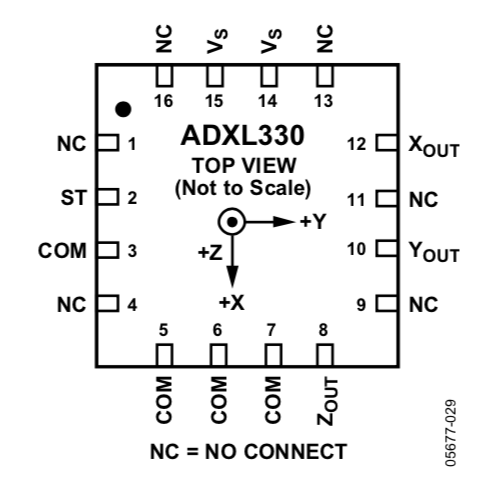
\includegraphics[width=4cm]{Images/ADXL330.png}
    \caption{Pin Configuration of ADXL330 \cite{ADXL330}}
    \label{fig:ADXL330}
\end{figure}

\vspace{-0.2cm} \noindent Using the accelerometer readings we calculate the pitch $(\theta)$ and yaw $(\psi)$ angles in radians with respect to the Kobuki axis orientation in Figure \ref{fig:kobuki} \cite{fisher_2011}.
Figures \ref{fig:pitch} and \ref{fig:yaw} indicate the angles in context of the Kobuki with both pitch and yaw angles showing increasing positive values. The resulting angle expressions in Eq.\ref{eq:accel_pitch} and Eq.\ref{eq:accel_yaw} are adapted from Fisher \cite{fisher_2011}. Note the yaw angle's arctan argument used in Eq.\ref{eq:accel_yaw} is defined instead of $\frac{x}{y}$ from Fisher \cite{fisher_2011}. Instead this argument is used to generate the same yaw behaviour in simulation as the myRIO mounting on the model has the $\pm x$, $\pm y$ and $\pm z$ axes swapped \cite[p.~235]{labguide}.
\begin{align}
    \theta &= \arccos \biggr( \frac{z}{\sqrt{x^2 + y^2 + z^2}} \biggr)\label{eq:accel_pitch}\\
    \psi &= \arctan(-\frac{y}{x})\label{eq:accel_yaw}
\end{align}
\vspace{-0.2cm}
\begin{figure}[H]
    \centering
    \begin{minipage}{0.45\textwidth}
    \centering
    \vspace{1cm}
    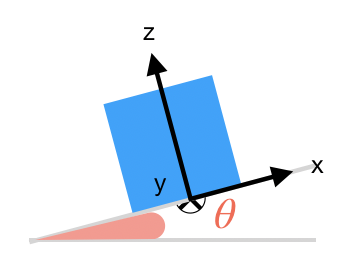
\includegraphics[width=3cm]{Images/Pitch.png}
    \caption{Positive pitch angle from 0, increasing in the direction of +z}
    \label{fig:pitch}
    \end{minipage}%
    \hspace{0.5cm}
    \begin{minipage}{0.45\textwidth}
    \centering
    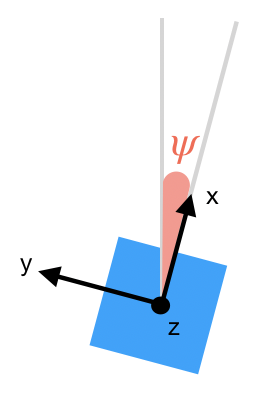
\includegraphics[width=2.2cm]{Images/Yaw.png}
    \caption{Positive yaw angle from 0, increasing in the direction of -y}
    \label{fig:yaw}
    \end{minipage}
\end{figure}

\subsubsection{Tuning Accelerometer Readings}\label{sec:accelerometer_LPF}
\vspace{-0.2cm} The typical output range for the accelerometer is $\pm 3.6g$ with a typical output voltage bias of 1.5V at 0$g$ and typical sensitivity of 300mV/$g$ for an operating range of 1.8 - 3.6V \cite{ADXL330}. The digital output received by the device will be $f(x) = 0.3x + 1.5$, rearranging this we get $x$ as the accelerometer reading in $g$,
\begin{align}
    x = \frac{f(x) - 1.5}{0.3}
\end{align}
With the level of sensitivity and fast sensor response rate, the accelerometer readings vary too frequently and may result in instability of robot performance. Therefore, we needed to use a low pass filter to average out the accelerometer reading so that it is accurate enough to represent the current state but also smooths out peak readings and avoids sensory overload. A discrete time solution would be ideal to implement on the digital system. A solution used in Ozyagcilar's paper was the exponential low pass filter, where the discrete time frequency transfer function is expressed in Eq.\ref{eq:LPF_freq} \cite[p.~16]{ozyagcilar}. It has a single pole on the real axis at $1 - \alpha$, where $\alpha$ represents the filter coefficient and should be smaller than 1 to keep the pole within the unit circle thereby guaranteeing system stability. 
\begin{align}
    H(z) &= \frac{\alpha}{1 - (1 -\alpha)z^{-1}}\label{eq:LPF_freq}
\end{align}
Expressing Eq.\ref{eq:LPF_freq} in the discrete time domain gives $y[n] = (1 - \alpha) y[n - 1] + \alpha x[n]$ \cite[p.~16]{ozyagcilar}. The difference equations describes the filter taking in a portion of the previous accelerometer reading and adding it to a corresponding proportion of the current reading. The filter would be used for each axis' reading independently before the smoothed output is used in Eq.\ref{eq:accel_pitch} and Eq.\ref{eq:accel_yaw} to calculate the pitch and yaw angles. The value of $\alpha$ was determined through experimentation on the live system.